\documentclass[final]{beamer}
%\documentclass[final,hyperref={pdfpagelabels=false}]{beamer} % beamer 3.07: get rid of beamer warnings
\mode<presentation> {  %% check http://www-i6.informatik.rwth-aachen.de/~dreuw/latexbeamerposter.php for examples
\usetheme{Cambridge}    %% you should define your own theme e.g. for big headlines using your own logos 
}
\usepackage{amsmath,amsthm, amssymb, latexsym}
\usefonttheme[onlymath]{serif}
%\boldmath

%\usepackage[size=custom,width=24in,height=16in,scale=1.2]{beamerposter}                       % e.g. for DIN-A0 poster
\usepackage[orientation=portrait,size=a0,scale=1]{beamerposter}                  % e.g. for DIN-A1 poster, with optional grid and debug output
%\usepackage[size=custom,width=200,height=120,scale=2,debug]{beamerposter}                     % e.g. for custom size poster
%\usepackage[orientation=portrait,size=a0,scale=1.0,printer=rwth-glossy-uv.df]{beamerposter}   % e.g. for DIN-A0 poster with rwth-glossy-uv printer check
% ...
%
  
%%%%%%%%%%%%%%%%%%%%%%%% Packages/includes
\usepackage[english]{babel}
%\usepackage[latin1]{inputenc}
\usepackage{times}
\usepackage{pgfpages}
\usepackage{pgfplotstable}
\usepackage{booktabs}
\usepackage[compatibility=false]{caption}
\usepackage{subcaption}

% Antonio's macros

\definecolor{accolornotes}{rgb}{0.7,0.3,0.2}
%\newcommand{\acnote}[1]{\textcolor{accolornotes}{[\textsc{ac:} {\bf #1}]}}
\newcommand{\acnote}[1]{\textcolor{accolornotes}{}}

\definecolor{changes}{rgb}{0.45,0,0}

\definecolor{yicolornotes}{rgb}{0.3,0.7,0.2}
%\newcommand{\yinote}[1]{\textcolor{yicolornotes}{[\textsc{yi:} {\bf #1}]}}
\newcommand{\yinote}[1]{\textcolor{yicolornotes}{}}

\definecolor{jscolornotes}{rgb}{0.7,0.3,0.7}
%\newcommand{\js}[1]{\textcolor{jscolornotes}{[\textsc{js:} {\bf #1}]}}
\newcommand{\js}[1]{\textcolor{jscolornotes}{}}

\definecolor{acgray}{rgb}{0.8,0.8,0.8}
\newcommand{\acremove}[1]{\textcolor{acgray}{[{#1}]}}

\definecolor{myred}{rgb}{0.6, 0, 0}
\definecolor{myblue}{rgb}{0.3, 0.1, 0.9}

%\definecolor{acgreen}{rgb}{0.1,0.5,0.1}
%\definecolor{acblue}{rgb}{0.1,0.1,0.5}
%\newcommand{\bl}[1]{\textcolor{acgreen}{#1}}
%\newcommand{\gr}[1]{\textcolor{acblue}{#1}}

\newcommand{\eg}{{\it e.g.}\ }
\newcommand{\ie}{{\it i.e.}\ }
\newcommand{\etal}{{\it et al.}\ }
\newcommand{\vs}{{v.s.}\ }
\newcommand{\cf}{{\it cf}\ }

\newcommand{\be}{\begin{equation}}
\newcommand{\ee}{\end{equation}}
\newcommand{\bea}{\begin{eqnarray}}
\newcommand{\eea}{\end{eqnarray}}
\newcommand{\beas}{\begin{eqnarray*}}
\newcommand{\eeas}{\end{eqnarray*}}

% Standardized section label and references
\newcommand{\chaplabel}[1]{\label{chap:#1}}
\newcommand{\chapref}[1]{\chaptername~\ref{chap:#1}} % Use mid-sentence
\newcommand{\Chapref}[1]{\chaptername~\ref{chap:#1}} % Use at start of sentence
\newcommand{\chaprefs}[2]{\chaptername s~\ref{chap:#1}~and~\ref{chap:#2}} % Use mid-sentence
\newcommand{\Chaprefs}[2]{\chaptername s~\ref{chap:#1}~and~\ref{chap:#2}} % Use at start of sentence
\newcommand{\appref}[1]{\appendixname~\ref{chap:#1}}

% Standardized section label and references
\newcommand{\seclabel}[1]{\label{sec:\reflabel-#1}}
\newcommand{\secref}[2][\reflabel]{Section~\ref{sec:#1-#2}} % Use mid-sentence
\newcommand{\Secref}[2][\reflabel]{Section~\ref{sec:#1-#2}} % Use at start of sentence
\newcommand{\secrefs}[3][\reflabel]{Sections~\ref{sec:#1-#2} and~\ref{sec:#1-#3}} % Use mid-sentence
\newcommand{\Secrefs}[3][\reflabel]{Sections~\ref{sec:#1-#2} and~\ref{sec:#1-#3}} % Use at start of sentence

% Standardized figure label and references
\newcommand{\figlabel}[2][\reflabel]{\label{fig:#1-#2}}
\newcommand{\figref}[2][\reflabel]{Figure~\ref{fig:#1-#2}} % Use mid-sentence
\newcommand{\Figref}[2][\reflabel]{Figure~\ref{fig:#1-#2}} % Use at start of sentence
\newcommand{\figrefs}[3][\reflabel]{Figures~\ref{fig:#1-#2} and~\ref{fig:#1-#3}} % Use mid-sentence
\newcommand{\Figrefs}[3][\reflabel]{Figures~\ref{fig:#1-#2} and~\ref{fig:#1-#3}} % Use at start of sentence

% Standardized table label and references
\newcommand{\tablelabel}[2][\reflabel]{\label{table:#1-#2}}
\newcommand{\tableref}[2][\reflabel]{Table~\ref{table:#1-#2}} % Use mid-sentence
\newcommand{\Tableref}[2][\reflabel]{Table~\ref{table:#1-#2}} % Use at start of sentence
\newcommand{\tablerefs}[3][\reflabel]{Tables~\ref{table:#1-#2} and~\ref{table:#1-#3}} % Use mid-sentence
\newcommand{\Tablerefs}[3][\reflabel]{Tables~\ref{table:#1-#2} and~\ref{table:#1-#3}} % Use at start of sentence

% Standardized equation label and references -- NB if you change this one, some of the uses in the text might have grammatical problems
\newcommand{\eqlabel}[1]{\label{eq:\reflabel-#1}}
\renewcommand{\eqref}[2][\reflabel]{(\ref{eq:#1-#2})} % Use mid-sentence
\newcommand{\Eqref}[2][\reflabel]{(\ref{eq:#1-#2})} % Use at start of sentence
\newcommand{\eqrefs}[3][\reflabel]{(\ref{eq:#1-#2}) and~(\ref{eq:#1-#3})} % Use mid-sentence
\newcommand{\Eqrefs}[3][\reflabel]{Equations (\ref{eq:#1-#2}) and~(\ref{eq:#1-#3})} % Use at start of sentence

% Standardized algorithm label and references
\newcommand{\alglabel}[2][\reflabel]{\label{alg:#1-#2}}
\newcommand{\algref}[2][\reflabel]{Algorithm~\ref{alg:#1-#2}} % Use mid-sentence
\newcommand{\algrefs}[3][\reflabel]{Algorithms~\ref{alg:#1-#2} and~\ref{alg:#1-#3}} % Use at start of sentence
\newcommand{\Algref}[2][\reflabel]{Algorithm~\ref{alg:#1-#2}} % Use mid-sentence
\newcommand{\Algrefs}[3][\reflabel]{Algorithm~\ref{alg:#1-#2} and~\ref{alg:#1-#3}} % Use at start of sentence

% Standardized part references
\newcommand{\PartI}{Part I\xspace}
\newcommand{\PartII}{Part II\xspace}
\newcommand{\PartIII}{Part III\xspace}


\newcommand{\reflabel}{dummy} % Dummy initial reflabel - use renewcommand at the start of each chapter

%%%
%%% Stuff for vector typesetting  ----------------------------------------
%%%
%%%    e.g. use "\v a" or "\v r" for vectors
%%%
\def\vec#1{\mathchoice{\mbox{\boldmath  $\displaystyle\bf#1$}}
{\mbox{\boldmath  $\textstyle\bf#1$}}
{\mbox{\boldmath  $\scriptstyle\bf#1$}}
{\mbox{\boldmath  $\scriptscriptstyle\bf#1$}}}
\def\v#1{\protect\vec #1}

%%%
%%% Stuff for matrix typesetting  ----------------------------------------
%%%
%%%    e.g. use "\m M" or "\m A" for matrices
%%%
\def\mat#1{\mathchoice{\mbox{\boldmath$\displaystyle\tt#1$}}
{\mbox{\boldmath$\textstyle\tt#1$}}
{\mbox{\boldmath$\scriptstyle\tt#1$}}
{\mbox{\boldmath$\scriptscriptstyle\tt#1$}}}
\def\m#1{\protect\mat #1}

%%%
%%% Stuff for bold maths typesetting  ----------------------------------------
%%%
%%%   e.g. use "\bfmu" for boldface mu symbol
%%%
\def\bfmu{\mbox{\boldmath$\mu$}}
\def\bftau{\mbox{\boldmath$\tau$}}
\def\bftheta{\mbox{\boldmath$\theta$}}
\def\bfdelta{\mbox{\boldmath$\delta$}}
\def\bfphi{\mbox{\boldmath$\phi$}}
\def\bfpsi{\mbox{\boldmath$\psi$}}
\def\bfeta{\mbox{\boldmath$\eta$}}
\def\bfnabla{\mbox{\boldmath$\nabla$}}
\def\bfGamma{\mbox{\boldmath$\Gamma$}}

%%%
%%% Stuff for argmax argmin  ----------------------------------------
%%%
\DeclareMathOperator*{\argmax}{argmax}
\DeclareMathOperator*{\argmin}{argmin}


%%%
%%% Stuff for calligraphic style  ----------------------------------------
%%%
\DeclareMathAlphabet{\mathcal}{OMS}{cmsy}{m}{n}

%% code to highlight maximal/minimal entries in column tables with pgftables
\newcommand{\findmax}[3]{
    \pgfplotstablevertcat{\datatable}{#1}
    \pgfplotstablecreatecol[
    create col/expr={%
    \pgfplotstablerow
    }]{rownumber}\datatable
    \pgfplotstablesort[sort key={#2},sort cmp={float >}]{\sorted}{\datatable}%
    \pgfplotstablegetelem{0}{rownumber}\of{\sorted}%
    \pgfmathtruncatemacro#3{\pgfplotsretval}
    \pgfplotstableclear{\datatable}
}

\newcommand{\findmin}[3]{
    \pgfplotstablevertcat{\datatable}{#1}
    \pgfplotstablecreatecol[
      create col/expr={%
    \pgfplotstablerow
    }]{rownumber}\datatable
    \pgfplotstablesort[sort key={#2},sort cmp={float <}]{\sorted}{\datatable}%
    \pgfplotstablegetelem{0}{rownumber}\of{\sorted}%
    \pgfmathtruncatemacro#3{\pgfplotsretval}
    \pgfplotstableclear{\datatable}
}

\pgfplotstableset{
    highlight col max/.code 2 args={
        \findmax{#1}{#2}{\maxval}
        \edef\setstyles{\noexpand\pgfplotstableset{
                every row \maxval\noexpand\space column #2/.style={
                    postproc cell content/.append style={
                        /pgfplots/table/@cell content/.add={$\noexpand\bf}{$}
                    },
                }
            }
        }\setstyles
    },
    highlight col min/.code 2 args={
        \findmin{#1}{#2}{\minval}
        \edef\setstyles{\noexpand\pgfplotstableset{
                every row \minval\noexpand\space column #2/.style={
                    postproc cell content/.append style={
                        /pgfplots/table/@cell content/.add={$\noexpand\bf}{$}
                    },
                }
            }
        }\setstyles
    },
    highlight row max/.code 2 args={
        \pgfmathtruncatemacro\rowindex{#2-1}
        \pgfplotstabletranspose{\transposed}{#1}
        \findmax{\transposed}{\rowindex}{\maxval}
        \edef\setstyles{\noexpand\pgfplotstableset{
                every row \rowindex\space column \maxval\noexpand/.style={
                    postproc cell content/.append style={
                        /pgfplots/table/@cell content/.add={$\noexpand\bf}{$}
                    },
                }
            }
        }\setstyles
    },
    highlight row min/.code 2 args={
        \pgfmathtruncatemacro\rowindex{#2-1}
        \pgfplotstabletranspose{\transposed}{#1}
        \findmin{\transposed}{\rowindex}{\maxval}
        \edef\setstyles{\noexpand\pgfplotstableset{
                every row \rowindex\space column \maxval\noexpand/.style={
                    postproc cell content/.append style={
                        /pgfplots/table/@cell content/.add={$\noexpand\bf}{$}
                    },
                }
            }
        }\setstyles
    },
}

\makeatletter
\long\def\pgfplotstabletypeset@opt@collectarg[#1]#2{%

    \pgfplotstable@isloadedtable{#2}%
        {\pgfplotstabletypeset@opt@[#1]{#2}}%
        {\pgfplotstabletypesetfile@opt@[#1]{#2}}%
}
\makeatother


\definecolor{filtercolor}{RGB}{255,230,153}
\definecolor{filtershade}{RGB}{205,185,123}
\definecolor{fmcolor}{RGB}{231,230,230}
\definecolor{fmshade}{RGB}{186,185,185}

\usepackage{tikz}
\usetikzlibrary{arrows,positioning,calc,tikzmark,decorations.pathreplacing}
%\usetikzlibrary{arrows,shapes,decorations.markings,calc,fadings}
\tikzstyle{every picture}+=[remember picture]

%\pgfdeclareimage{shield}{shieldbw}
%\begin{tikzfadingfrompicture}[name=shieldfading,inner sep=0]
%  \node [fill=transparent!0,opacity=0.3,rotate=45,scale=25] {\pgfuseimage{shield}};
%\end{tikzfadingfrompicture}

%\usebackgroundtemplate{%
%\begin{tikzpicture}[inner sep=0]
 % Watermark using transparent image 
  %  \node[fill=transparent!0,opacity=0.1,rotate=45,scale=25,anchor=west] {\pgfuseimage{shield}};
 
 % Watermark using fadings 
  %\node[fill=white,minimum width=\paperwidth,minimum height=\paperheight,anchor=west]{};
  % fill the same region with yellow but using a fading as mask
  %\path[scope fading=shieldfading,fit fading=true];
  %\node[fill=CambridgeCoreTeal,minimum width=\paperwidth,minimum height=\paperheight,anchor=west]{};
%\end{tikzpicture}
%}

\captionsetup[figure]{labelformat=empty}
\captionsetup[table]{labelformat=empty}

%%%%%%%%%%%%%%%%%%%%%%%% Bibliography
\usepackage[backend=bibtex,style=ieee,natbib=true,url=false,doi=false]{biblatex}
%\AtEveryCitekey{\iffootnote{\color{black}\tiny}{\color{black}}}
\addbibresource{../references.bib}
  
\newcommand{\covarlabels}[5]{%
\begin{tikzpicture}[anchor=south west]
    \node [inner sep=0pt] (c)
    {
        #5
    };
    \ifx\covarwidth\undefined
    \newlength{\covarwidth}
    \newlength{\covarheight}
    \fi
    \settowidth{\covarwidth}{#5}
    \settoheight{\covarheight}{#5}
    \path[use as bounding box] (c.south west) rectangle (c.north east);
    \node [anchor=south west, xshift=-0.5em, yshift=-0.5em, rotate=45] at (c.north west) {\footnotesize 0};
    \node [anchor=south east, xshift=\covarwidth, yshift=-0.2em] at (c.north west) {\footnotesize #4};
    \node [anchor=south west, xshift=0.25em, yshift=-1.05\covarheight, rotate=90] at (c.north west) {\footnotesize #2};
    \node [anchor=south, xshift=0.5\covarwidth] at (c.north west) {\footnotesize\texttt{#3}};
    \node [anchor=south, xshift=0.2em, yshift=-0.5\covarheight, rotate=90] at (c.north west) {\footnotesize \texttt{#1}};
\end{tikzpicture}%
}
  
%%%%%%%%%%%%%%%%%%%%%%%% Title Page Setup
\title % (optional, use only with long paper titles)
{Deep Roots}
\subtitle{Improving CNN Efficiency with Hierarchical Filter Groups}

\author[Y. Ioannou, D. Robertson, R. Cipolla and A. Criminisi]
{Yani Ioannou\inst{1} \and Duncan Robertson\inst{2} \and Roberto Cipolla\inst{1} \and Antonio Criminisi\inst{2}}

\institute[University of Cambridge and Microsoft Research] % (optional, but mostly needed)
{\inst{1} University of Cambridge, \inst{2} Microsoft Research, Cambridge}

\date

\begin{document}

%\addtobeamertemplate{headline}{} 
%{
%\begin{tikzpicture}[remember picture,overlay] 
%\node [shift={(-10 cm,-5cm)}] at (current page.north east) {
\includegraphics[height=3cm]{uc-rev-cmyk}}; 
%\end{tikzpicture} 
%}

%%%%%%%%%%%%%%%%%%%%%%%%%%%%%%%%%%%%%%%%%%%%%%%%%%%%%%%%%%%%%%%%%%%%%%%%%%%%%%%%%%%%%%%%%%%%%%%

%%%%%%%%%%%%%%%%%%%%
\begin{frame}{}

\begin{columns}[t]

\begin{column}{0.32\paperwidth}

\begin{block}{Summary}
  \begin{itemize}
	\item We train CNNs with `root modules', a novel sparse connection structure that resembles a tree root
    \item In effect our networks learn a basis for the channel extents of filters, based on compact filter groups
	\item Our models are \alert{faster} and use \alert{fewer parameters}, while maintaining \alert{accuracy}
      \item For \alert{ResNet 50}, our model has \alert{40\%} fewer parameters, \alert{45\%} fewer FLOPS, and is 31\% (12\%) faster on a CPU (GPU)
      \item For \alert{ResNet 200}, our model has \alert{44\%} fewer parameters and \alert{25\%} fewer FLOPS
      \item For GoogLeNet, our model has 7\% fewer parameters and is 21\% (16\%) faster on a CPU (GPU)
  \end{itemize}
\end{block}

\begin{block}{Previous Work: Learning a Basis Space for Filters}{}
\begin{itemize}
   \item In \citep{Ioannou2016}, linear combination of low-rank filters is learned, \ie a basis space for filters:
\end{itemize}

\vspace{1em}

\begin{figure}
   \includegraphics[width=0.9\textwidth, page=3]{../figs/sparsification}
\end{figure}

\vspace{1em}

\begin{itemize}
    \item A set of filters of different shape (similar to `Inception', but low-rank and of different orientation~\cite{Szegedy2014going})
    \item On the following layer, use $d\times [1 \times 1 \times m]$ filters to linearly combine
    \item Only learning a low-rank filter in the spatial dimensions -- filters maintain full channel depth
\end{itemize}
\end{block}

\begin{block}{Filter Groups}

\begin{figure}[t]
\begin{subfigure}[t]{0.65\linewidth}
\centering
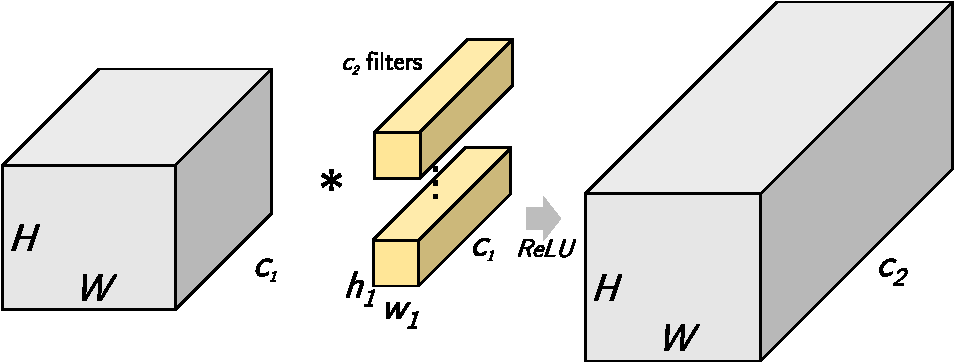
\includegraphics[width=0.9\linewidth, page=1]{../figs/groupfig}
    \caption{Convolution.}
   \label{fig:normalconv}
\end{subfigure}
~
\begin{subfigure}[t]{0.65\linewidth}
\centering
\includegraphics[width=0.9\linewidth, page=2]{../figs/groupfig}
   \caption{Convolution with filter groups.}
   \label{fig:groupedconv}
\end{subfigure}
\label{fig:groupconfig}
\end{figure}
\begin{itemize}
    \item Convolutional filters (yellow) typically have the same channel dimension ($c_1$) as the input feature maps (gray)
    \item With convolutional filter groups~\citep{Krizhevsky2012}, $g$ independent groups of $c_2/g$ filters operate on a fraction $c_1/g$ of the input feature map channels
    \item This reduces filter dimensions from $h$$\times$$w$$\times$$c_1$ to $h$$\times$$w$$\times$$c_1/g$
    \item This change does not affect the dimensions of the input and output feature maps but significantly reduces computational complexity and the number of model parameters.
\end{itemize}
\end{block}


\begin{block}{Root Module}
\begin{figure}[t]
\centering
\begin{subfigure}[b]{0.95\linewidth}
\centering
\includegraphics[width=\linewidth, page=4]{../figs/groupfig}
   \caption{Convolution with $d$ filters of shape $h\times w\times c$.}
   \label{fig:normalresnet}
\end{subfigure}\\
\begin{subfigure}[b]{0.95\linewidth}
\includegraphics[width=\linewidth, page=5]{../figs/groupfig}
   \caption{Root-2 Module: $d$ filters in $g = 2$ filter groups, of shape $h\times w\times c/2$.}
   \label{fig:rootresnet2}
\end{subfigure}
\begin{subfigure}[b]{0.95\linewidth}
\includegraphics[width=\linewidth, page=6]{../figs/groupfig}
   \caption{Root-4 Module: $d$ filters in $g = 4$ filter groups, of shape $h\times w\times c/4$.}
   \label{fig:rootresnet4}
\end{subfigure}
%\caption{\textbf{Root Modules.} Root modules (b), (c) compared to a typical set of convolutional layers (a) found in ResNet and other modern architectures. Grey blocks represent the feature maps over which a layer's filters operate, while colored blocks represent the filters of each layer. 
%}
\label{fig:rootmodule}
\end{figure}
\begin{itemize}
    \item (a) shows the typical set of conv.\ layers found in ResNet and other modern architectures
    \item Root modules (b), (c) have a given number of filter groups, with fewer connections to the previous layer's outputs
    \item Spatial convolutional layer is followed by a 1$\times$1 convolution. Like in \citep{Ioannou2016}, this learns a linear combination of the basis filters (filter groups), implicitly representing a filter of full channel depth, but with limited filter dependence.
\end{itemize}
\end{block}
\end{column}

\begin{column}{0.66\paperwidth}

\begin{block}{Root: Network-in-Network}

\begin{figure}[t]
\begin{subfigure}[t]{0.9\linewidth}
\hspace*{-2cm}
\begin{tikzpicture}
    \begin{scope}[]
     \matrix[column sep=0em, ampersand replacement=\&]{
     \node (1a) {
        \raisebox{-0.5\height}{\includegraphics[height=0.08\linewidth, page=15]{../figs/groupfig}}
     };\&
    \node (1b) {
        \raisebox{-0.5\height}{\includegraphics[height=0.11\linewidth, page=17]{../figs/groupfig}}
    };\&
    \node (1c) {
        \raisebox{-0.5\height}{\includegraphics[height=0.11\linewidth, page=17]{../figs/groupfig}}
    };\&
    \node (2a) {
        \raisebox{-0.5\height}{\includegraphics[height=0.09\linewidth, page=16]{../figs/groupfig}}
    };\&
    \node (2b) {
        \raisebox{-0.5\height}{\includegraphics[height=0.11\linewidth, page=17]{../figs/groupfig}}
    };\&
    \node (2c) {
        \raisebox{-0.5\height}{\includegraphics[height=0.11\linewidth, page=17]{../figs/groupfig}}
    };\&
    \node (3a) {
        \raisebox{-0.5\height}{\includegraphics[height=0.09\linewidth, page=16]{../figs/groupfig}}
    };\&
    \node (3b) {
        \raisebox{-0.5\height}{\includegraphics[height=0.11\linewidth, page=17]{../figs/groupfig}}
    };\&
    \node (3c) {
        \raisebox{-0.5\height}{\includegraphics[height=0.11\linewidth, page=17]{../figs/groupfig}}
    };\&
    \node (7) {
        {\LARGE$\cdots$}
    };\\
    \draw node{{\footnotesize \textit{input image}} \hspace{0.7em} {\footnotesize \textit{conv1a}}};\&
    \draw node{\footnotesize \textit{conv1b}};\&
    \draw node{\footnotesize \textit{conv1c}};\&
    \draw node{\footnotesize \textit{conv2a}};\&
    \draw node{\footnotesize \textit{conv2b}};\&
    \draw node{\footnotesize \textit{conv2c}};\&
    \draw node{\footnotesize \textit{conv3a}};\&
    \draw node{\footnotesize \textit{conv3b}};\&
    \draw node{\footnotesize \textit{conv3c}};\\
     };
    \end{scope}
\end{tikzpicture}
    \caption{Standard}
    \label{fig:standardtopology}
\end{subfigure}
~
\begin{subfigure}[t]{0.9\linewidth}
\hspace*{-2cm}
\begin{tikzpicture}
    \begin{scope}[]
    \matrix[column sep=0em, ampersand replacement=\&]{
    \node (1a) {
        \includegraphics[height=0.08\linewidth, page=15]{../figs/groupfig}
    };\&
    \node (1b) {
        \includegraphics[height=0.11\linewidth, page=17]{../figs/groupfig}
    };\& 
    \node (1c) {
        \includegraphics[height=0.11\linewidth, page=17]{../figs/groupfig}
    };\& 
    \node (2a) {
        \includegraphics[height=0.15\linewidth, page=19]{../figs/groupfig}
    };\&
    \node (2b) {
        \includegraphics[height=0.11\linewidth, page=17]{../figs/groupfig}
    };\&
    \node (2c) {
        \includegraphics[height=0.11\linewidth, page=17]{../figs/groupfig}
    };\&
    \node (3a) {
        \includegraphics[height=0.09\linewidth, page=18]{../figs/groupfig}
    };\&
    \node (3b) {
        \includegraphics[height=0.11\linewidth, page=17]{../figs/groupfig}
    };\&
    \node (3c) {
        \includegraphics[height=0.11\linewidth, page=17]{../figs/groupfig}
    };\&
    \node (4) {
        {\LARGE$\cdots$}
    };\\
    };
    \draw[decorate,decoration={brace,mirror},](2a.south west) -- node[below=3pt] {\small root-4 module} ++(10, 0);
    \draw[decorate,decoration={brace,mirror},yshift=-2em](3a.south west) + (0, -1.5) -- node[below=3pt] {\small root-2 module} ++(10.5, -1.5);
    \end{scope}
\end{tikzpicture}
\caption{Root-4 Architecture}
\label{fig:root4topology}
\end{subfigure}
\end{figure}
\end{block}

\vspace{-1.1em}
\begin{columns}[t]
\begin{column}{0.32\paperwidth}


\begin{block}{Results: Network-in-Network (CIFAR10)}

\begin{table}[t]
\footnotesize
\begin{subtable}[b]{0.48\linewidth}
\caption{\textbf{Filter groups per layer}}
\label{table:ninconfig}
%\resizebox{\linewidth}{!}{
\begin{tabular}{@{}lm{1.2em}m{1.2em}m{1.2em}m{1.2em}m{1.2em}m{1.2em}m{1.2em}m{1.2em}m{1.2em}@{}}
\toprule
    Model & \multicolumn{3}{c}{conv1} & \multicolumn{3}{c}{conv2} & \multicolumn{3}{c}{conv3} \\
%     & \textit{\footnotesize a} & \textit{\footnotesize b} & \textit{\footnotesize c} & \textit{\footnotesize a} & \textit{\footnotesize b} & \textit{\footnotesize c} & \textit{\footnotesize a} & \textit{\footnotesize b} & \textit{\footnotesize c} \\
     & \textit{\tiny5$\times$5} & \textit{\tiny1$\times$1} & \textit{\tiny1$\times$1} & \textit{\tiny5$\times$5} & \textit{\tiny1$\times$1} & \textit{\tiny1$\times$1} & \textit{\tiny3$\times$3} & \textit{\tiny1$\times$1} & \textit{\tiny1$\times$1} \\
    \midrule
    Orig. & 1 & 1 & 1 & 1 & 1 & 1 & 1 & 1 & 1\\
    \midrule
    root-2 & 1 & 1 & 1 & 2 & 1 & 1 & 1 & 1 & 1\\
    root-4 & 1 & 1 & 1 & 4 & 1 & 1 & 2 & 1 & 1\\
    root-8 & 1 & 1 & 1 & 8 & 1 & 1 & 4 & 1 & 1\\
    root-16 & 1 & 1 & 1 & 16 & 1 & 1 & 8 & 1 & 1\\
    \bottomrule
\end{tabular}
%}
\end{subtable}
\begin{subtable}[b]{0.48\linewidth}
\caption{\textbf{Results}}
\label{table:nincifarresults}
\pgfplotstableread[col sep=comma]{../rootdata/nincifar.csv}\data
\pgfplotstableread[col sep=comma]{../rootdata/nincifar_root_s.csv}\codata
\pgfplotstablevertcat{\data}{\codata}
%\resizebox{\linewidth}{!}{
\pgfplotstabletypeset[
    every head row/.style={
    before row=\toprule,after row=\midrule},
    every last row/.style={
    after row=\bottomrule},
    every first row/.style={
    after row=\midrule}, 
    fixed zerofill,     % Fill numbers with zeros
    columns={full name, ma, param, accuracy, cpu, gpu},
    columns/full name/.style={
        column name=Model,
        string type
    },
    columns/ma/.style={
        column name=FLOPS {\small $\times 10^{8}$},
        preproc/expr={{##1/1e8}}
    },
    columns/param/.style={
        column name=Param. {\small $\times 10^{5}$},
        preproc/expr={{##1/1e5}}
    },
    columns/accuracy/.style={
        column name=Acc.,
        precision=4
    },
    columns/gpu/.style={
        column name=GPU (ms),
        precision=3
    },
    columns/cpu/.style={
        column name=CPU (ms),
        precision=1
    },
%    column type/.add={@{}lrrrrrr@{}}{},
    column type/.add={@{}lp{3em}p{3em}p{3em}p{3em}p{3em}p{3em}@{}}{},
    highlight col max ={\data}{accuracy},
    highlight col min ={\data}{param}, 
    highlight col min ={\data}{ma}, 
    col sep=comma]{\data}
%}
\end{subtable}
\end{table}
\begin{figure}[t]
\footnotesize
\begin{subfigure}[t]{0.49\linewidth}
\pgfplotstableread[col sep=comma]{../rootdata/nincifar.csv}\datatable
\pgfplotstableread[col sep=comma]{../rootdata/nincifar_root_s.csv}\rdatatable
\pgfplotsset{major grid style={dotted,red}}

\begin{tikzpicture}
%\tikzstyle{every node}=[font=\footnotesize]
\begin{axis}[
  width=0.95\linewidth,
  height=0.5\linewidth,
  axis x line=bottom,
  ylabel=Error,
  xlabel=Model Parameters,
  axis lines=left,
  enlarge x limits=0.05,
  enlarge y limits=0.05,
  grid=major,
  %xmin=0,
  ytick={0.002,0.004,...,1.0},
  ymin=0.075,ymax=0.088,
  x label style={at={(axis description cs:0.5,-0.13)},anchor=north},
  y label style={at={(axis description cs:-0.05,.5)},anchor=south},
  xticklabel style={
        /pgf/number format/fixed,
        /pgf/number format/precision=1
  },
  yticklabel={\pgfmathparse{\tick*1}\pgfmathprintnumber{\pgfmathresult}\%},style={
        /pgf/number format/fixed zerofill,
        /pgf/number format/precision=1
  },
  legend style={at={(1.2,1.2)}, anchor=south east, column sep=0.2em},
  legend columns=4,
]
\addplot[mark=*,mark options={fill=red},
   %nodes near coords,
   only marks,
   point meta=explicit symbolic,
   error bars/y dir=both,
   error bars/y fixed=0.00131497782,
] table[meta=name,x=param,y expr={1 - \thisrow{accuracy} },]{\datatable};
\addplot[mark=square*,mark options={fill=green},
   nodes near coords, only marks,
   every node near coord/.append style={inner sep=4pt},
   point meta=explicit symbolic,
] table[meta=name,x=param,y expr={1 - \thisrow{accuracy} },]{\rdatatable};
\legend{NiN, Root}
\end{axis}
\end{tikzpicture}
%\caption{\textbf{Model Parameters \vs Error.}}
%\label{fig:nincifarparamconvonly}
\end{subfigure}
~
\begin{subfigure}[t]{0.49\linewidth}
\pgfplotstableread[col sep=comma]{../rootdata/nincifar.csv}\datatable
\pgfplotstableread[col sep=comma]{../rootdata/nincifar_root_s.csv}\rdatatable
\pgfplotsset{major grid style={dotted,red}}

\begin{tikzpicture}
%\tikzstyle{every node}=[font=\footnotesize]
\begin{axis}[
  width=0.95\linewidth,
  height=0.5\linewidth,
  axis x line=bottom,
  %ylabel=Error,
  xlabel=FLOPS (Multiply-Add),
  axis lines=left,
  enlarge x limits=0.05,
  enlarge y limits=0.05,
  grid=major,
  %xmin=0,
  ytick={0.002,0.004,...,1.0},
  x label style={at={(axis description cs:0.5,-0.13)},anchor=north},
  y label style={at={(axis description cs:-0.05,.5)},anchor=south},
  ymin=0.075,ymax=0.088,
  xticklabel style={
        /pgf/number format/fixed zerofill,
        /pgf/number format/precision=1
  },
  yticklabel={\pgfmathparse{\tick*1}\pgfmathprintnumber{\pgfmathresult}\%},style={
        /pgf/number format/fixed zerofill,
        /pgf/number format/precision=1
  },
]
\addplot[mark=*,mark options={fill=red},
   %nodes near coords,
   only marks,
   point meta=explicit symbolic,
   error bars/y dir=both,
   error bars/y fixed=0.00131497782,
] table[meta=name,x=ma,y expr={1 - \thisrow{accuracy} },]{\datatable};
\addplot[mark=square*,mark options={fill=green},
   nodes near coords, only marks,
   every node near coord/.append style={inner sep=4pt},
   point meta=explicit symbolic,
] table[meta=name,x=ma,y expr={1 - \thisrow{accuracy} },]{\rdatatable};
\end{axis}
\end{tikzpicture}
%\caption{\textbf{FLOPS (Multiply-Add) \vs Error.}}
%\label{fig:nincifarmaconvonly}
\end{subfigure}

\caption{\textbf{Network-in-Network CIFAR10 Results.} Spatial filters (3$\times$3, 5$\times$5) are grouped hierarchically. The best models are closest to the origin. For the standard network, the mean and standard deviation (error bars) are shown over 5 different random initializations.
%(left) Parameters \vs Error, (right) FLOPS \vs Error.
}
\label{fig:nincifarplotsconvonly}
\end{figure}

\end{block}

\begin{block}{Results: ResNet 50 (Imagenet)}
\begin{table}[t]
\footnotesize
\begin{subtable}[b]{0.48\linewidth}
\caption{\textbf{Filter groups per layer}}
\label{table:resnet50config}
\centering
\begin{tabular}{@{}lm{1.1em}m{1.1em}m{1.1em}m{1.1em}m{1.1em}m{1.1em}m{1.1em}m{1.1em}m{1.1em}m{1.1em}m{1.1em}m{1.1em}@{}}
%\begin{tabular}{@{}lcccccccccccc@{}}
\toprule
    Model &{\tiny conv1} & \multicolumn{2}{c}{\tiny res2\{a--c\}} & \multicolumn{2}{c}{\tiny res3\{a--d\}} & \multicolumn{2}{c}{\tiny res4\{a--f\}} & \multicolumn{2}{c}{\tiny res5\{a--c\}} \\
     & \textit{\tiny7$\times$7} & \textit{\tiny1$\times$1} & \textit{\tiny3$\times$3} & \textit{\tiny1$\times$1} & \textit{\tiny3$\times$3} & \textit{\tiny1$\times$1} & \textit{\tiny3$\times$3} & \textit{\tiny1$\times$1} & \textit{\tiny3$\times$3} \\
    \midrule
    Orig. & 1 & 1 & 1 & 1 &  1 & 1 &  1 & 1 & 1 \\
    \midrule
    root-2 & 1 & 1 & 2 & 1 &  1 & 1 &  1 & 1 & 1 \\
    root-4 & 1 & 1 & 4 & 1 &  2 & 1 &  1 & 1 & 1 \\
    root-8 & 1 & 1 & 8 & 1 &  4 & 1 &  2 & 1 & 1 \\
    root-16 & 1 & 1 & 16 & 1 &  8 & 1 &  4 & 1 & 2 \\
    root-32 & 1 & 1 & 32 & 1 & 16 & 1 &  8 & 1 & 4 \\
    root-64 & 1 & 1 & 64 & 1 & 32 & 1 & 16 & 1 & 8 \\
    \bottomrule
\end{tabular}
\end{subtable}
\begin{subtable}[b]{0.48\linewidth}
\caption{\textbf{Results}}
\label{table:resnet50imagenetresults}
%\resizebox{\linewidth}{!}{
\centering
\pgfplotstableread[col sep=comma]{../data/resnet50ma.csv}\data
\pgfplotstableread[col sep=comma]{../data/resnet50maconvonly.csv}\codata
\pgfplotstablevertcat{\data}{\codata}
\pgfplotstableset{
    create on use/singlegpu/.style={
        create col/expr={\thisrow{GPU Forward} / \thisrow{Batch Size}}},
}
\pgfplotstableset{
    create on use/singlecpu/.style={
        create col/expr={\thisrow{CPU Forward} / \thisrow{Batch Size}}},
}
\pgfplotstabletypeset[
    every head row/.style={
    before row=\toprule,after row=\midrule},
    every last row/.style={
    after row=\bottomrule},
    every first row/.style={
    after row=\midrule}, 
    fixed zerofill,     % Fill numbers with zeros
    columns={Full Name, Multiply-Acc., Param., Top-1 Acc., Top-5 Acc., singlecpu, singlegpu},
    columns/Full Name/.style={
        column name=Model,
        string type
    },
    columns/singlegpu/.style={
        column name=GPU (ms),
        precision=1
    },
    columns/singlecpu/.style={
        column name=CPU (ms),
        precision=0
    },
    columns/Multiply-Acc./.style={
        column name=FLOPS {\small $\times 10^{9}$},
        preproc/expr={{##1/1e9}}
    },
    columns/Param./.style={
        column name=Param. {\small $\times 10^{7}$},
        preproc/expr={{##1/1e7}}
    },
    columns/Top-1 Acc./.style={precision=3},
    columns/Top-5 Acc./.style={precision=3},
    highlight col max ={\data}{Top-1 Acc.},
    highlight col max ={\data}{Top-5 Acc.}, 
    highlight col min ={\data}{Param.}, 
    highlight col min ={\data}{Multiply-Acc.}, 
    column type/.add={@{}lp{2.9em}p{2.5em}p{2.5em}p{2.5em}p{2.1em}p{2.1em}@{}}{},
    col sep=comma]{\data}
%}
\end{subtable}
\end{table}
\begin{figure}[t]
\footnotesize
\begin{subfigure}[b]{0.48\linewidth}
\pgfplotstableread[col sep=comma]{../data/resnet50ma.csv}\gdatatable
\pgfplotstableread[col sep=comma]{../data/resnet50maconvonly.csv}\codatatable
\pgfplotsset{major grid style={dotted,red}}

\pgfplotstableset{
    create on use/singlecpu/.style={
        create col/expr={\thisrow{CPU Forward} / \thisrow{Batch Size}}},
}

\begin{tikzpicture}
\begin{axis}[
  width=\linewidth,
  height=0.45\linewidth,
  axis x line=bottom,
  ylabel=Top-5 Error,
  xlabel=Model Parameters (\# Floats),
  axis lines=left,
  enlarge x limits=0.05,
  %enlarge y limits=0.1,
  grid=major,
  %xmin=0,
  x label style={at={(axis description cs:0.5,-0.13)},anchor=north},
  y label style={at={(axis description cs:0.0,.5)},anchor=south},
  ytick={0.01,0.02,...,0.2},
  ymin=0.07,ymax=0.1,
  xticklabel style={
        /pgf/number format/fixed,
        /pgf/number format/precision=3
  },
  yticklabel={\pgfmathparse{\tick*100}\pgfmathprintnumber{\pgfmathresult}\%},style={
        /pgf/number format/fixed,
        /pgf/number format/precision=1
  },
  legend style={at={(1.3,1.25)}, anchor=north east, column sep=0.5em},
  legend columns=3,
]
\addplot[mark=*,mark options={fill=red},
   %nodes near coords,
   only marks,
   point meta=explicit symbolic,
] table[meta=Network,x=Param.,y expr={1 - \thisrow{Top-5 Acc.} },]{\gdatatable};
\addplot[mark=square*,mark options={fill=green},
   nodes near coords, nodes near coords align = {below}, only marks,
   every node near coord/.append style={inner sep=4pt},
   only marks,
   point meta=explicit symbolic,
] table[meta=Network,x=Param.,y expr={1 - \thisrow{Top-5 Acc.} },]{\codatatable};
\legend{ResNet 50, All Filters, Spatial Filters, LDE Half}
\end{axis}
\end{tikzpicture}
\caption{\textbf{Model Param.\ \vs Top-5 Error.}}
\label{fig:resnet5050param}
\end{subfigure}
~
\begin{subfigure}[b]{0.48\linewidth}
\pgfplotstableread[col sep=comma]{../data/resnet50ma.csv}\gdatatable
\pgfplotstableread[col sep=comma]{../data/resnet50maconvonly.csv}\codatatable
\pgfplotsset{major grid style={dotted,red}}

\begin{tikzpicture}
\begin{axis}[
  width=\linewidth,
  height=0.45\linewidth,
  axis x line=bottom,
  %ylabel=Top-5 Error,
  xlabel=FLOPS (Multiply-Add),
  axis lines=left,
  enlarge x limits=0.05,
  %enlarge y limits=0.1,
  grid=major,
  %xmin=0,
  x label style={at={(axis description cs:0.5,-0.13)},anchor=north},
  y label style={at={(axis description cs:-0.05,.5)},anchor=south},
  ytick={0.01,0.02,...,0.2},
  ymin=0.07,ymax=0.1,
  xticklabel style={
        /pgf/number format/fixed,
        /pgf/number format/precision=3
  },
  yticklabel={\pgfmathparse{\tick*100}\pgfmathprintnumber{\pgfmathresult}\%},style={
        /pgf/number format/fixed,
        /pgf/number format/precision=1
  },
  legend style={at={(0.98,0.98)}, anchor=north east, column sep=0.5em},
  legend columns=3,
]
\addplot[mark=*,mark options={fill=red},
   %nodes near coords,
   only marks,
   point meta=explicit symbolic,
] table[meta=Network,x=Multiply-Acc.,y expr={1 - \thisrow{Top-5 Acc.} },]{\gdatatable};
\addplot[mark=square*,mark options={fill=green},
   nodes near coords, nodes near coords align = {below}, only marks,
   every node near coord/.append style={inner sep=4pt},
   only marks,
   point meta=explicit symbolic,
] table[meta=Network,x=Multiply-Acc.,y expr={1 - \thisrow{Top-5 Acc.} },]{\codatatable};
\end{axis}
\end{tikzpicture}
\caption{\textbf{FLOPS \vs Top-5 Error.}}
\label{fig:resnet50ma}
\end{subfigure}
~
\begin{subfigure}[b]{0.48\linewidth}
\pgfplotstableread[col sep=comma]{../data/resnet50ma.csv}\gdatatable
\pgfplotstableread[col sep=comma]{../data/resnet50maconvonly.csv}\codatatable
\pgfplotsset{major grid style={dotted,red}}

\centering
\begin{tikzpicture}
\begin{axis}[
  width=\linewidth,
  height=0.45\linewidth,
  axis x line=bottom,
  ylabel=Top-5 Error,
  xlabel=GPU Forward (ms),
  axis lines=left,
  enlarge x limits=0.05,
  %enlarge y limits=0.1,
  grid=major,
  %xmin=0,
  x label style={at={(axis description cs:0.5,-0.13)},anchor=north},
  y label style={at={(axis description cs:0.0,.5)},anchor=south},
  ytick={0.01,0.02,...,0.2},
  ymin=0.07,ymax=0.1,
  xticklabel style={
        /pgf/number format/fixed,
        /pgf/number format/precision=3
  },
  yticklabel={\pgfmathparse{\tick*100}\pgfmathprintnumber{\pgfmathresult}\%},style={
        /pgf/number format/fixed,
        /pgf/number format/precision=1
  },
  legend style={at={(0.98,0.98)}, anchor=north east, column sep=0.5em},
  legend columns=3,
]
\addplot[mark=*,mark options={fill=red},
   %nodes near coords,
   only marks,
   point meta=explicit symbolic,
] table[meta=Network,
    x expr={\thisrow{GPU Forward} / \thisrow{Batch Size}},
    y expr={1 - \thisrow{Top-5 Acc.} }
]{\gdatatable};
\addplot[mark=square*,mark options={fill=green},
   nodes near coords, nodes near coords align = {below}, only marks,
   every node near coord/.append style={inner sep=4pt},
   only marks,
   point meta=explicit symbolic,
] table[meta=Network,
    x expr={\thisrow{GPU Forward} / \thisrow{Batch Size}},
    y expr={1 - \thisrow{Top-5 Acc.} },
]{\codatatable};
%\legend{ResNet 50, All Filters, Spatial Filters}
\end{axis}
\end{tikzpicture}
\caption{\textbf{GPU Forward \vs Top-5 Error.}}
\label{fig:resnet5050gpuforward}
\end{subfigure}
~
\begin{subfigure}[b]{0.48\linewidth}
\pgfplotstableread[col sep=comma]{../data/resnet50ma.csv}\gdatatable
\pgfplotstableread[col sep=comma]{../data/resnet50maconvonly.csv}\codatatable
\pgfplotsset{major grid style={dotted,red}}

\centering
\begin{tikzpicture}
\begin{axis}[
  width=\linewidth,
  height=0.45\linewidth,
  axis x line=bottom,
  %ylabel=Top-5 Error,
  xlabel=CPU Forward (ms),
  axis lines=left,
  enlarge x limits=0.05,
  %enlarge y limits=0.1,
  grid=major,
  %xmin=0,
  x label style={at={(axis description cs:0.5,-0.13)},anchor=north},
  y label style={at={(axis description cs:-0.05,.5)},anchor=south},
  ytick={0.01,0.02,...,0.2},
  ymin=0.07,ymax=0.1,
  xticklabel style={
        /pgf/number format/fixed,
        /pgf/number format/precision=3
  },
  yticklabel={\pgfmathparse{\tick*100}\pgfmathprintnumber{\pgfmathresult}\%},style={
        /pgf/number format/fixed,
        /pgf/number format/precision=1
  },
  legend style={at={(0.98,0.98)}, anchor=north east, column sep=0.5em},
  legend columns=3,
]
\addplot[mark=*,mark options={fill=red},
   %nodes near coords,
   only marks,
   point meta=explicit symbolic,
] table[meta=Network,
    x expr={\thisrow{CPU Forward} / \thisrow{Batch Size}},
    y expr={1 - \thisrow{Top-5 Acc.} },
]{\gdatatable};
\addplot[mark=square*,mark options={fill=green},
   nodes near coords, nodes near coords align = {below}, only marks,
   every node near coord/.append style={inner sep=4pt},
   only marks,
   point meta=explicit symbolic,
] table[meta=Network,
    x expr={\thisrow{CPU Forward} / \thisrow{Batch Size}},
    y expr={1 - \thisrow{Top-5 Acc.} },
]{\codatatable};
%\legend{ResNet 50, All Filters, Spatial Filters}
\end{axis}
\end{tikzpicture}
\caption{\textbf{CPU Forward \vs Top-5 Error.}}
\label{fig:resnet5050cpuforward}
\end{subfigure}

\caption{\textbf{ResNet-50 Results.} Models with filter groups have fewer parameters, and less floating point operations, while maintaining error comparable to the baseline.}
\label{fig:resnet50plots}
\end{figure}

\end{block}


\begin{block}{Results: ResNet 200 (Imagenet)}
\begin{table}[t]
\footnotesize
\caption{\textbf{Results}}
\label{table:resnet200imagenetresults}
%\resizebox{\columnwidth}{!}{
\centering
\pgfplotstableread[col sep=comma]{../data/resnet200.csv}\data
\pgfplotstabletypeset[
    every head row/.style={
    before row=\toprule,after row=\midrule},
    every last row/.style={
    after row=\bottomrule},
    every first row/.style={
    after row=\midrule}, 
    columns={full name, ma, param, top1, top5},
    columns/full name/.style={
        column name=Model,
        string type
    },
    columns/ma/.style={
        column name=FLOPS~{\small$\times 10^{12}$},
        fixed zerofill,
        preproc/expr={{##1/1e12}},
    },
    columns/param/.style={
        column name=Param.~{\small$\times 10^{7}$},
        fixed zerofill,
        preproc/expr={{##1/1e7}},
    },
    columns/top1/.style={
        precision=4,
        column name=Top-1 Err.,
        fixed zerofill,
    },
    columns/top5/.style={
        precision=4,
        column name=Top-5 Err.,
        fixed zerofill,
    },
    column type/.add={@{}lrrrrrr@{}}{},
    highlight col min ={\data}{top1},
    highlight col min ={\data}{top5}, 
    highlight col min ={\data}{param}, 
    highlight col min ={\data}{ma}, 
    col sep=comma]{\data}
%}
\end{table}
\begin{itemize}
\item Recently these results were extended upon by \citep{2016arXiv161105431X} to improve the accuracy of ResNet significantly, in ResNeXt, which placed 2nd in the ILSVRC 2016 challenge.
\end{itemize}
\end{block}

\begin{block}{More Information}
\vspace{-1em}
\begin{center}
    \tikz\node[opacity=1, anchor=north]{\includegraphics[width=0.06\textheight]{qrcodeblue}};
\end{center}
\end{block}
\end{column}

%%%%%%%%%%%%%%%%%%%%%%%%%%%%%%%%%%%%%%%%%%%%%%%%%%%%%%%%%%%%%%%%%%%%%%%%%%%%%%%%%%%%%%%%%%%%%%%
\begin{column}{0.32\paperwidth}

\begin{block}{Analysis: Inter-Layer Response Covariance}
\begin{figure}[t]
\centering
\begin{subfigure}[c]{0.48\linewidth}
\centering
    \covarlabels{conv2c}{192}{conv3a}{192}{\includegraphics[width=0.5\linewidth]{../figs/ninroot32/layercovar_conv8-pdf.pdf}}
    \caption{Non-whitened}
    \label{fig:notwhitened}
\end{subfigure}
~
\begin{subfigure}[c]{0.48\linewidth}
\centering
    \covarlabels{conv2c}{192}{conv3a}{192}{\includegraphics[width=0.5\linewidth]{../figs/ninroot32/layercovarwhite_conv8-pdf.pdf}}
    \caption{Whitened responses}
    \label{fig:whitened}
\end{subfigure}
\caption{Inter-layer covariance of root-32 NiN model}
\label{fig:whitevsnot}
\end{figure}
\begin{itemize}
\item To show the dependencies between filters on adjacent layers, we show the covariance between responses of the layers over the training set.
\item However, without whitening the responses of each layer, these are conflated with existing covariances from the data/other layers
%\item Instead, the (absolute) covariance of the whitened responses for the training set are shown
\end{itemize}
\end{block}

\begin{block}{Analysis: Network-in-Network}
\begin{figure}[t]
\begin{subfigure}[c]{0.46\linewidth}
    \covarlabels{conv2c}{192}{conv2c}{192}{\includegraphics[width=0.45\textwidth]{../figs/nin/corrcoef_conv6-pdf.pdf}}
~
    \covarlabels{conv3a}{192}{conv3a}{192}{\includegraphics[width=0.45\textwidth]{../figs/nin/corrcoef_conv8-pdf.pdf}}
\label{fig:corrroot1}
\caption{\textbf{Network-in-Network}}
\vspace*{0.6em}
\end{subfigure}
~
\begin{subfigure}[c]{0.46\linewidth}
    \covarlabels{conv2c}{192}{conv2c}{192}{\includegraphics[width=0.45\textwidth]{../figs/ninroot4/corrcoef_conv6-pdf.pdf}}
~
    \covarlabels{conv3a}{192}{conv3a}{192}{\includegraphics[width=0.45\textwidth]{../figs/ninroot4/corrcoef_conv8-pdf.pdf}}
\caption{\textbf{Root-4}}
\vspace*{0.6em}
\label{fig:corrroot4}
\end{subfigure}
~
\begin{subfigure}[c]{0.46\linewidth}
    \covarlabels{conv2c}{192}{conv2c}{192}{\includegraphics[width=0.45\textwidth]{../figs/ninroot8/corrcoef_conv6-pdf.pdf}}
~
    \covarlabels{conv3a}{192}{conv3a}{192}{\includegraphics[width=0.45\textwidth]{../figs/ninroot8/corrcoef_conv8-pdf.pdf}}
\caption{\textbf{Root-8}}
\vspace*{0.6em}
\label{fig:corrroot8}
\end{subfigure}
~
\begin{subfigure}[c]{0.46\linewidth}
    \covarlabels{conv2c}{192}{conv2c}{192}{\includegraphics[width=0.45\textwidth]{../figs/ninroot32/corrcoef_conv6-pdf.pdf}}
~
    \covarlabels{conv3a}{192}{conv3a}{192}{\includegraphics[width=0.45\textwidth]{../figs/ninroot32/corrcoef_conv8-pdf.pdf}}
\caption{\textbf{Root-32}}
\label{fig:corrroot32}
\end{subfigure}
\centering
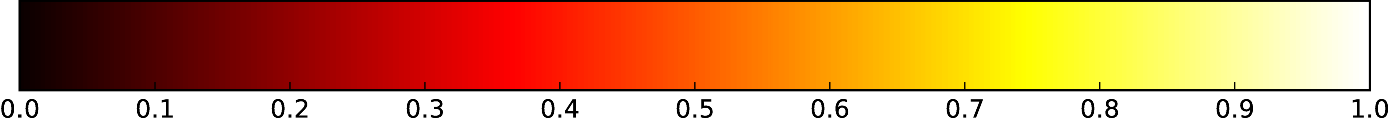
\includegraphics[width=0.4\linewidth]{../figs/colorbar}
\caption{\textbf{Intra-Layer Correlation.} Absolute Correlation of filters within each layer.}
\label{fig:nincorr}
\end{figure}

\begin{figure}[t]
\centering
\begin{subfigure}[b]{0.3\linewidth}
\centering
    \covarlabels{conv2c}{192}{conv3a}{192}{\includegraphics[width=\textwidth]{../figs/msrc-cifar-nin-4pad-conv8-corr-pdf.pdf}}
    \caption{Standard}
    \label{fig:normalcovartestfull}
\end{subfigure}
~
\begin{subfigure}[b]{0.3\linewidth}
\centering
    \covarlabels{conv2c}{192}{conv3a}{192}{\includegraphics[width=\linewidth]{../figs/msrc-cifar-nin-4pad-funnel2-convonly-conv8-corr-pdf.pdf}}
    \caption{Root-2}
    \label{fig:root2corrfull}
\end{subfigure}
~
\begin{subfigure}[b]{0.3\linewidth}
\centering
    \covarlabels{conv2c}{192}{conv3a}{192}{\includegraphics[width=\linewidth]{../figs/msrc-cifar-nin-4pad-funnel4-convonly-conv8-corr-pdf.pdf}}
    \caption{Root-4}
    \label{fig:root4corrfull}
\end{subfigure}
~
\begin{subfigure}[b]{0.3\linewidth}
\centering
    \vspace*{0.6em}
    \covarlabels{conv2c}{192}{conv3a}{192}{\includegraphics[width=\linewidth]{../figs/msrc-cifar-nin-4pad-funnel8-convonly-conv8-corr-pdf.pdf}}
    \caption{Root-8}
    \label{fig:root8corrfull}
\end{subfigure}
~
\begin{subfigure}[b]{0.3\linewidth}
\centering
    \vspace*{0.6em}
    \covarlabels{conv2c}{192}{conv3a}{192}{\includegraphics[width=\linewidth]{../figs/msrc-cifar-nin-4pad-funnel16-convonly-conv8-corr-pdf.pdf}}
    \caption{Root-16}
    \label{fig:root16corrfull}
\end{subfigure}
~
\begin{subfigure}[b]{0.3\linewidth}
\centering
    \vspace*{0.6em}
    \covarlabels{conv2c}{192}{conv3a}{192}{\includegraphics[width=\linewidth]{../figs/msrc-cifar-nin-4pad-funnel32-convonly-conv8-corr-pdf.pdf}}
    \caption{Root-32}
    \label{fig:root32corrfull}
\end{subfigure}
\caption{\textbf{Filter Inter-layer Covariance conv2c--conv3a}}
\label{fig:covarfull}
\end{figure}
\begin{itemize}
\item The block-diagonal sparsity learned by a root module is visible in the correlation of filters on layers \texttt{conv3a} and \texttt{conv2c} in the NiN network
\item Rather than a random appearing structure of dependence seen in (a), root modules have more structured dependence, where well correlated filters are grouped close to the related filters on the previous layer
\end{itemize}
\end{block}

\begin{block}{References}
{
\renewcommand*{\bibfont}{\scriptsize}
%\vspace{-1em}
\printbibliography
}
\end{block}

%\tikz\node[opacity=0.6, anchor=north] at (current page.center){\includegraphics[width=15em]{qrcodeblue}};

\end{column}

\end{columns}
\end{column}
\end{columns}
%%%%%%%%%%%%%%%%%%%%%%%%%%%%%%%%%%%%%%%%%%%%%%%%%%%%%%%%%%%%%%%%%%%%%%%%%%%%%%%%%%%%%%%%%%%%%%%

\end{frame}

\end{document}

